\subsection{Ускорительный комплекс FAIR}\label{sec:secFAIR}

% Диссер Ольги Дереновской

% The Compressed Baryonic Matter experiment
% Sélim SEDDIKI
% 10.1051/ epjconf / 201 4 7100120

% http://localhost/Lib/r126c.pdf

Европейский центр по исследованиям с помощью тяжёлых ионов и антипротонов (Facility for Antiproton and Ion Research, FAIR, \cite{FAIR}) строится в пригороде Дармштадта в Германии.
%Это будет исследовательский ускорительный комплекс нового поколения, не имеющий аналогов в мире и открывающий уникальные возможности для проведения научных исследований по наиболее актуальным направлениям современной науки и технологий.
Он предоставит высокоэнергетичные, прецизионно настроенные пучки антипротонов и различных ионов от водорода до урана с беспрецедентным качеством и интенсивностью.
%\textbf{Эти пучки заряженных частиц будут потом ускорены и использованы при создании новых, часто очень экзотических частиц для ряда параллельных экспериментальных программ, одной из которых является плотная барионная материя (Compressed Baryonic Matter, CBM).}
Научная программа на ускорительном комплексе FAIR охватывает следующие направления:
\begin{itemize}
\item исследование в рамках коллаборации CBM уравнения состояния ядерной материи, получаемой в столкновениях тяжелых ионов;
\item изучение структуры ядра и исследования в области ядерной астрофизики с использованием пучков как стабильных ионов, так и радиоактивных ионов в рамках направления NUSTAR~\cite{NUSTAR};
\item изучение структуры адронов, исследования, направленные на развитие теории сильных взаимодействий с использованием пучков антипротонов в рамках коллаборации PANDA~\cite{PANDA};
\item исследования в области физики сверхплотной плазмы, атомной физики, квантовой электродинамики в сверхсильных электромагнитных полях, прикладные исследования с пучками ионов для радиационного материаловедения, медицины и биологии в рамках направления APPA~\cite{APPA}.
\end{itemize}

%Коллаборации, планирующие исследования на FAIR, разделены на 4 группы:
%\begin{itemize}
%\item структура ядра и ядерная астрофизика --- NuSTAR (Nuclear STructure, Astrophysics and Reactions);
%\item плотная барионная материя --- CBM (Compressed Baryonic Matter);
%\item антипротонная программа --- PANDA (antiProton ANnihilation in DArmstadt);
%\item физика сверхплотной плазмы, атомная физика, а также прикладные исследования по материаловедению и биологии --- APPA (Atomic, Plasma Physics and Applications).
%\end{itemize}

На \figref{fig:FAIRstructure} приведена планируемая схема ускорительного комплекса FAIR рядом с существующей инфраструктурой институтa тяжёлоионных исследований (Gesellschaft f\"{u}r Schwerionenforschung, GSI).
%\textbf{FAIR предоставит уникальные возможности для исследования фазовой диаграммы КХД при экстремально высоких плотностях барионной материи наряду с многими другими областями исследований --- адронная физика с антипротоновым пучком, физика ядерных структур с радиоактивным пучком, плазма-физика с высоко-импульсным ядерным пучком.}
Центральный элемент комплекса --- двойной синхротрон тяжёлых ионов SIS100/300 (SchwerIonenSynchrotron) длиной 1100~м. В качестве инжектора пучка в SIS100/300 будут выступать существующие в GSI универсальный линейный ускоритель UNILAC (UNIversal Linear ACcelarator) и далее синхротрон SIS18.
%Также FAIR включает в себя:
%сверхпроводящий магнитный сепаратор фрагментов Super-FRS (Super Fragment Separator),
%накопительное кольцо высоких энергий HESR (High Energy Storage Ring),
%коллекторное кольцо CR (Collector Ring),
%рециркуляционное экспериментальное накопительное кольцо RESR (Recirculation Experimental Storage Ring), 
%при наличии дополнительного финансирования --- новое экспериментальное накопительное кольцо NESR (New Experimental Storage Ring),
%коплекс для исследования низкоэнергетичных антипротонов и тяжёлых ионов FLAIR (Facility for Low-energy Antiproton and heavy Ion Research).

\begin{figure}[H]
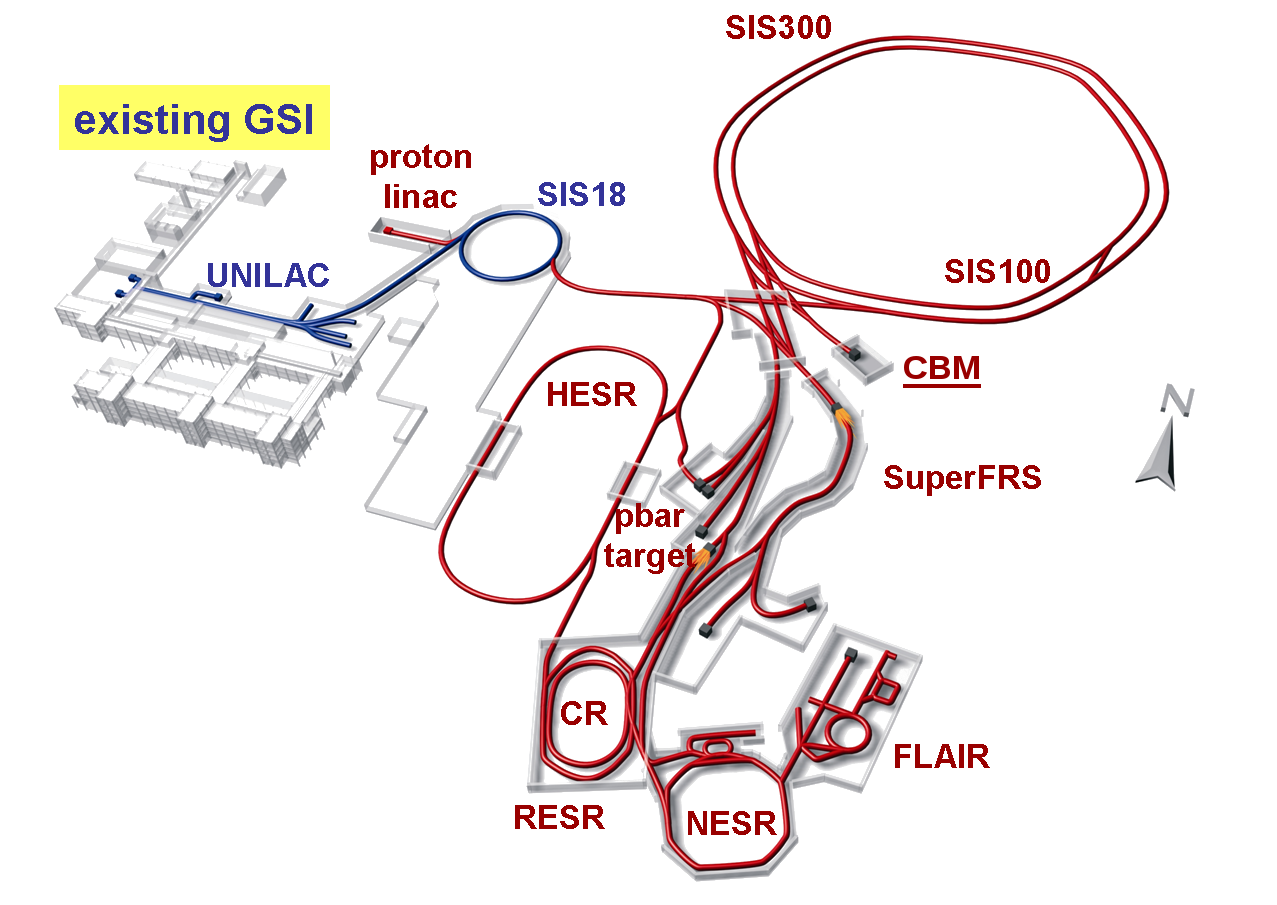
\includegraphics[width=1.0\textwidth]{pictures/FAIR_structure.png}
\caption{Схема комплекса FAIR. Super-FRS --- Super Fragment Separator, HESR --- High Energy Storage Ring, CR --- Collector Ring, RESR --- Recirculation Experimental Storage Ring, NESR --- New Experimental Storage Ring, FLAIR --- Facility for Low-energy Antiproton and heavy Ion Research.}
\label{fig:FAIRstructure}
\end{figure}

Синхротроны SIS100 и SIS300 будут иметь магнитную жёсткость 100~Тл$\cdot$м и 300~Тл$\cdot$м соответственно. В первой фазе FAIR будет реализован только SIS100. Этот ускоритель будет способен производить пучки ионов максимальной зарядности от протона до урана с интенсивностью до $10^9$ ионов в секунду и энергией от~2~до~11~\GeVperNucl{} для самых тяжёлых ионов ($Au$, $Pb$, $U$), до 17~\GeVperNucl{} для более лёгких ионов ($Z/A=0.5$) и до 35~\GeV{} для протонов.
Ещё одной отличительной особенностью FAIR являтся то, что он будет предоставлять пучок для нескольких (до~4) исследовательских установок одновременно, позволяя экспериментаторам работать с пучком до 4~месяцев в год.

%CBM работать с пучком тяжёлых ионов до 4~месяцев в год. На \figref{fig:FAIRstructure3} показан%а схема предоставления пучка параллельно нескольким экспериментам. \\
%\textbf{Описание можно стырить из FAIR BTR.}

%\begin{figure}[H]
%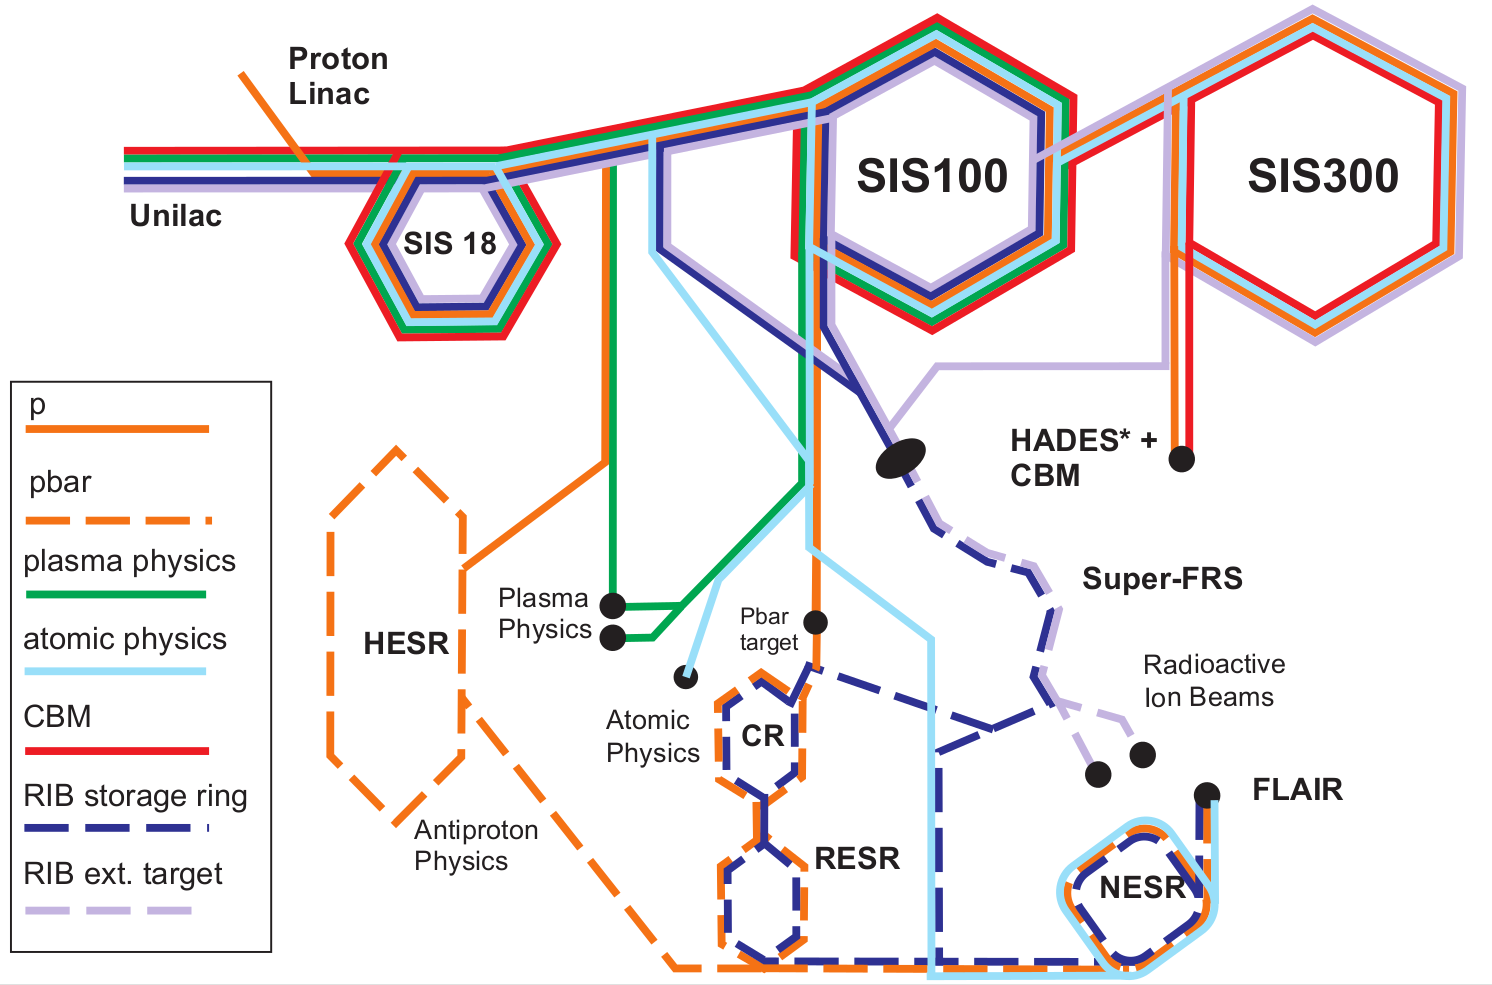
\includegraphics[width=1.0\textwidth]{pictures/FAIR_structure_3.png}
%\caption{Схема комплекса FAIR.}
%\label{fig:FAIRstructure3}
%\end{figure}

%Широкий диапазон энергий, предоставляемый FAIR, позволит производить ядерную материю при максимальных плотностях, доступных при столкновениях тяжёлых ионов. В соответствии с разными моделями ядерного взаимодействия на раннем этапе центрального $Au+Au$ столкновения при энергии пучка 20~\GeVperNucl{} ($s_{NN} \approx 6.4$~\GeVperNucl{}) плотность в центре сгустка будет достигать уровня примерно в 12~раз выше обычной ядерной плотности.

%\small{The broad energy range provided by FAIR will allow producing nuclear matter at the maximal net baryon density achievable with heavy ion collisions [8]. As shown in Figure 3, according to various transport models, the density reaches up to about twelve times the normal nuclear matter density in the core and at the early stage of central $Au+Au$ collisions at a beam energy of 20 GeV/nucleon ($s_{NN}$ $\approx$ 6.4 GeV). As can be seen in Figure 4, this important feature of the FAIR accelerator is supported by the derived chemical freeze-out parameters that are required to reproduce, within a canonical or grand canonical statistical model, the measured particle yields in central $A+A$ collisions at SIS, AGS, SPS and RHIC energies ($s_{NN}$ $\approx$ 2, 5, 20, 200 GeV, respectively) [9]. As the beam energy decreases a clear shift towards lower temperatures and higher $\mu_{B}$ occurs.}

%\small{The identification of multi-strange hyperons, hypernuclei, particles with charm quarks and vector mesons decaying into lepton pairs requires efficient background suppression and very high interaction rates. In order to select events containing those rare observables, the tracks of each collision have to be reconstructed and filtered online with respect to physical signatures. This concept represents a paradigm shift for data taking in high-energy physics experiments: CBM will run without hierarchical trigger system. Self-triggered read-out electronics, a high-speed data processing and acquisition system, fast algorithms, and, last but not least, radiation hard detectors are indispensable prerequisites for a successful operation of the experiment.}